% Template LaTeX document for CSSR4Africa Deliverables
% Adapted from documents prepared by EPFL for the RobotCub project
% and subsequently by the University of Skövde for the DREAM project
%
% DV 28/06/2023

\documentclass{CSSRforAfrica}

\usepackage[hidelinks,colorlinks=false]{hyperref}
\usepackage[titletoc,title]{appendix}
\usepackage{latexsym}

%%%%%%%%%%%%%%%%%%%%%%%%%%%%%%%%%%%%%%%%%%%%%%%%%%%%%%%%%%%%%%%%
\usepackage{dirtree}  %% DV: added to display the website directory structure
\usepackage{listings} %% DV: added for listings
\usepackage{subcaption} %% DV: added for captions in listings
%%%%%%%%%%%%%%%%%%%%%%%%%%%%%%%%%%%%%%%%%%%%%%%%%%%%%%%%%%%%%%%%
%%% for listings %%%%%%%%%%%%%%%%%%%%%%%%%%%%%%%%%%%%%%%%%%%%%%%%%%%%
\captionsetup[figure]{format=hang}
\usepackage{xcolor}
\definecolor{codegreen}{rgb}{0,0.6,0}
\definecolor{codegray}{rgb}{0.5,0.5,0.5}
\definecolor{codepurple}{rgb}{0.58,0,0.82}
\definecolor{backcolour}{rgb}{0.95,0.95,0.92}


\lstdefinestyle{Numbering}{
    backgroundcolor=\color{backcolour},   
    commentstyle=\color{codegreen},
    keywordstyle=\color{magenta},
    numberstyle=\tiny\color{codegray},
    stringstyle=\color{codepurple},
    basicstyle=\ttfamily\small,
    breakatwhitespace=false,         
    breaklines=true,                 
    captionpos=b,                    
    keepspaces=true,                 
    numbers=left,                    
    numbersep=5pt,                  
    showspaces=false,                
    showstringspaces=false,
    showtabs=false,                  
    tabsize=2
}

\lstdefinestyle{withoutNumbering}{
    backgroundcolor=\color{backcolour},   
    commentstyle=\color{codegreen},
    keywordstyle=\color{magenta},
    stringstyle=\color{codepurple},
    basicstyle=\ttfamily\small,
    breakatwhitespace=false,         
    breaklines=true,                 
    captionpos=b,                    
    keepspaces=true,                 
    showspaces=false,                
    showstringspaces=false,
    showtabs=false,                  
    tabsize=2
}
%%%%%%%%%%%%%%%%%%%%%%%%%%%%%%%%%%%%%%%%%%%%%%%%%%%

\newcommand{\blank}{~\\}
\newcommand{\checkbox}{{~~~~~~~\leavevmode \put(-7,-1.5){  \huge $\Box$  }}}

\begin{document}
\input{epsf}

%%
%% SHOULD NOT NEED TO BE CHANGED BEFORE THIS POINT
%% ------------------------------------------------
%%

\deliverable{D7.1}     
\title{D7.1 Online Presence}    

\leadpartner{Carnegie Mellon University Africa }             
\partner{The University of the Witwatersrand}                        

\revision{1.1}               
\deliverabledate{01/10/2023}   
\submissiondate{03/08/2023}  
\revisiondate{07/08/2023}   
\disseminationlevel{PU}
\responsible{D. Vernon }       


%%
%% Create the titlepage
%%

\maketitle
 

\section*{Executive Summary}
%===============================================================
\label{executive_summary}
%%\addcontentsline{toc}{section}{Executive Summary}
 
The objective of the task associated with this deliverable is to communicate project aims and results to the general public and stakeholders.  
The deliverable takes the form of a website, a wiki, and a report.  The  operational launch of the initial version of the website and wiki, and this report which describes these initial versions, is scheduled for completion at month 3. The website and the wiki will be maintained throughout the duration of the project.

 The website is primarily a forum for disseminating information about the project to a broader audience, e.g., goals of the project, information about the consortium, project work plan, deliverables, publications, and project news.
The wiki is primarily a forum for exchanging information among the partners in the project consortium. The majority of the material available on it is concerned with the effective operation of the project, e.g., meetings, reports, references, and templates.
The website domain name is {\small \url {www.cssr4africa.org}} and is hosted on GitHub. The wiki is also hosted on GitHub and it is linked from the website. It can also be accessed directly from the CSSR4Africa repository.

Software developed in the project can be accessed by cloning the CSSR4Africa repository on GitHub, i.e., Deliverable D7.3. Instructions on how to install the software can be found in Deliverable D3.3.  
\newpage


 
 
%\graphicspath{{./figs/}}
\pagebreak
\tableofcontents
\newpage


\section{Introduction}
%===============================================================
There are three elements to the online presence of the CSSR4Africa project: a website, a wiki, and a software repository. This deliverable documents the creation and maintenance of the website and wiki; Deliverable 7.3 documents the creation and maintenance of the software repository.

The website is a forum that is used to inform any interested party about the project, its goals, its progress, and its results.  The wiki is a forum intended to be used mainly by the partners in the CSSR4Africa consortium.  Both wiki and website are public.



\section{CSSR4Africa Website}
%----------------------

\subsection{Domain Name}
%----------------------
The website domain name is {\small \url {www.cssr4africa.org}}.  The domain name is registered with Hostway.  The domain name {\small \url {www.cssr4africa.com}} has also been registered to avoid  cyber-squatting for the purposes of extortion, i.e., publishing undesirable material on a website with the same domain name but with a different top-level domain.

\subsection{Website Structure}
%------------------------


\begin{figure}[tb]
\begin{center}
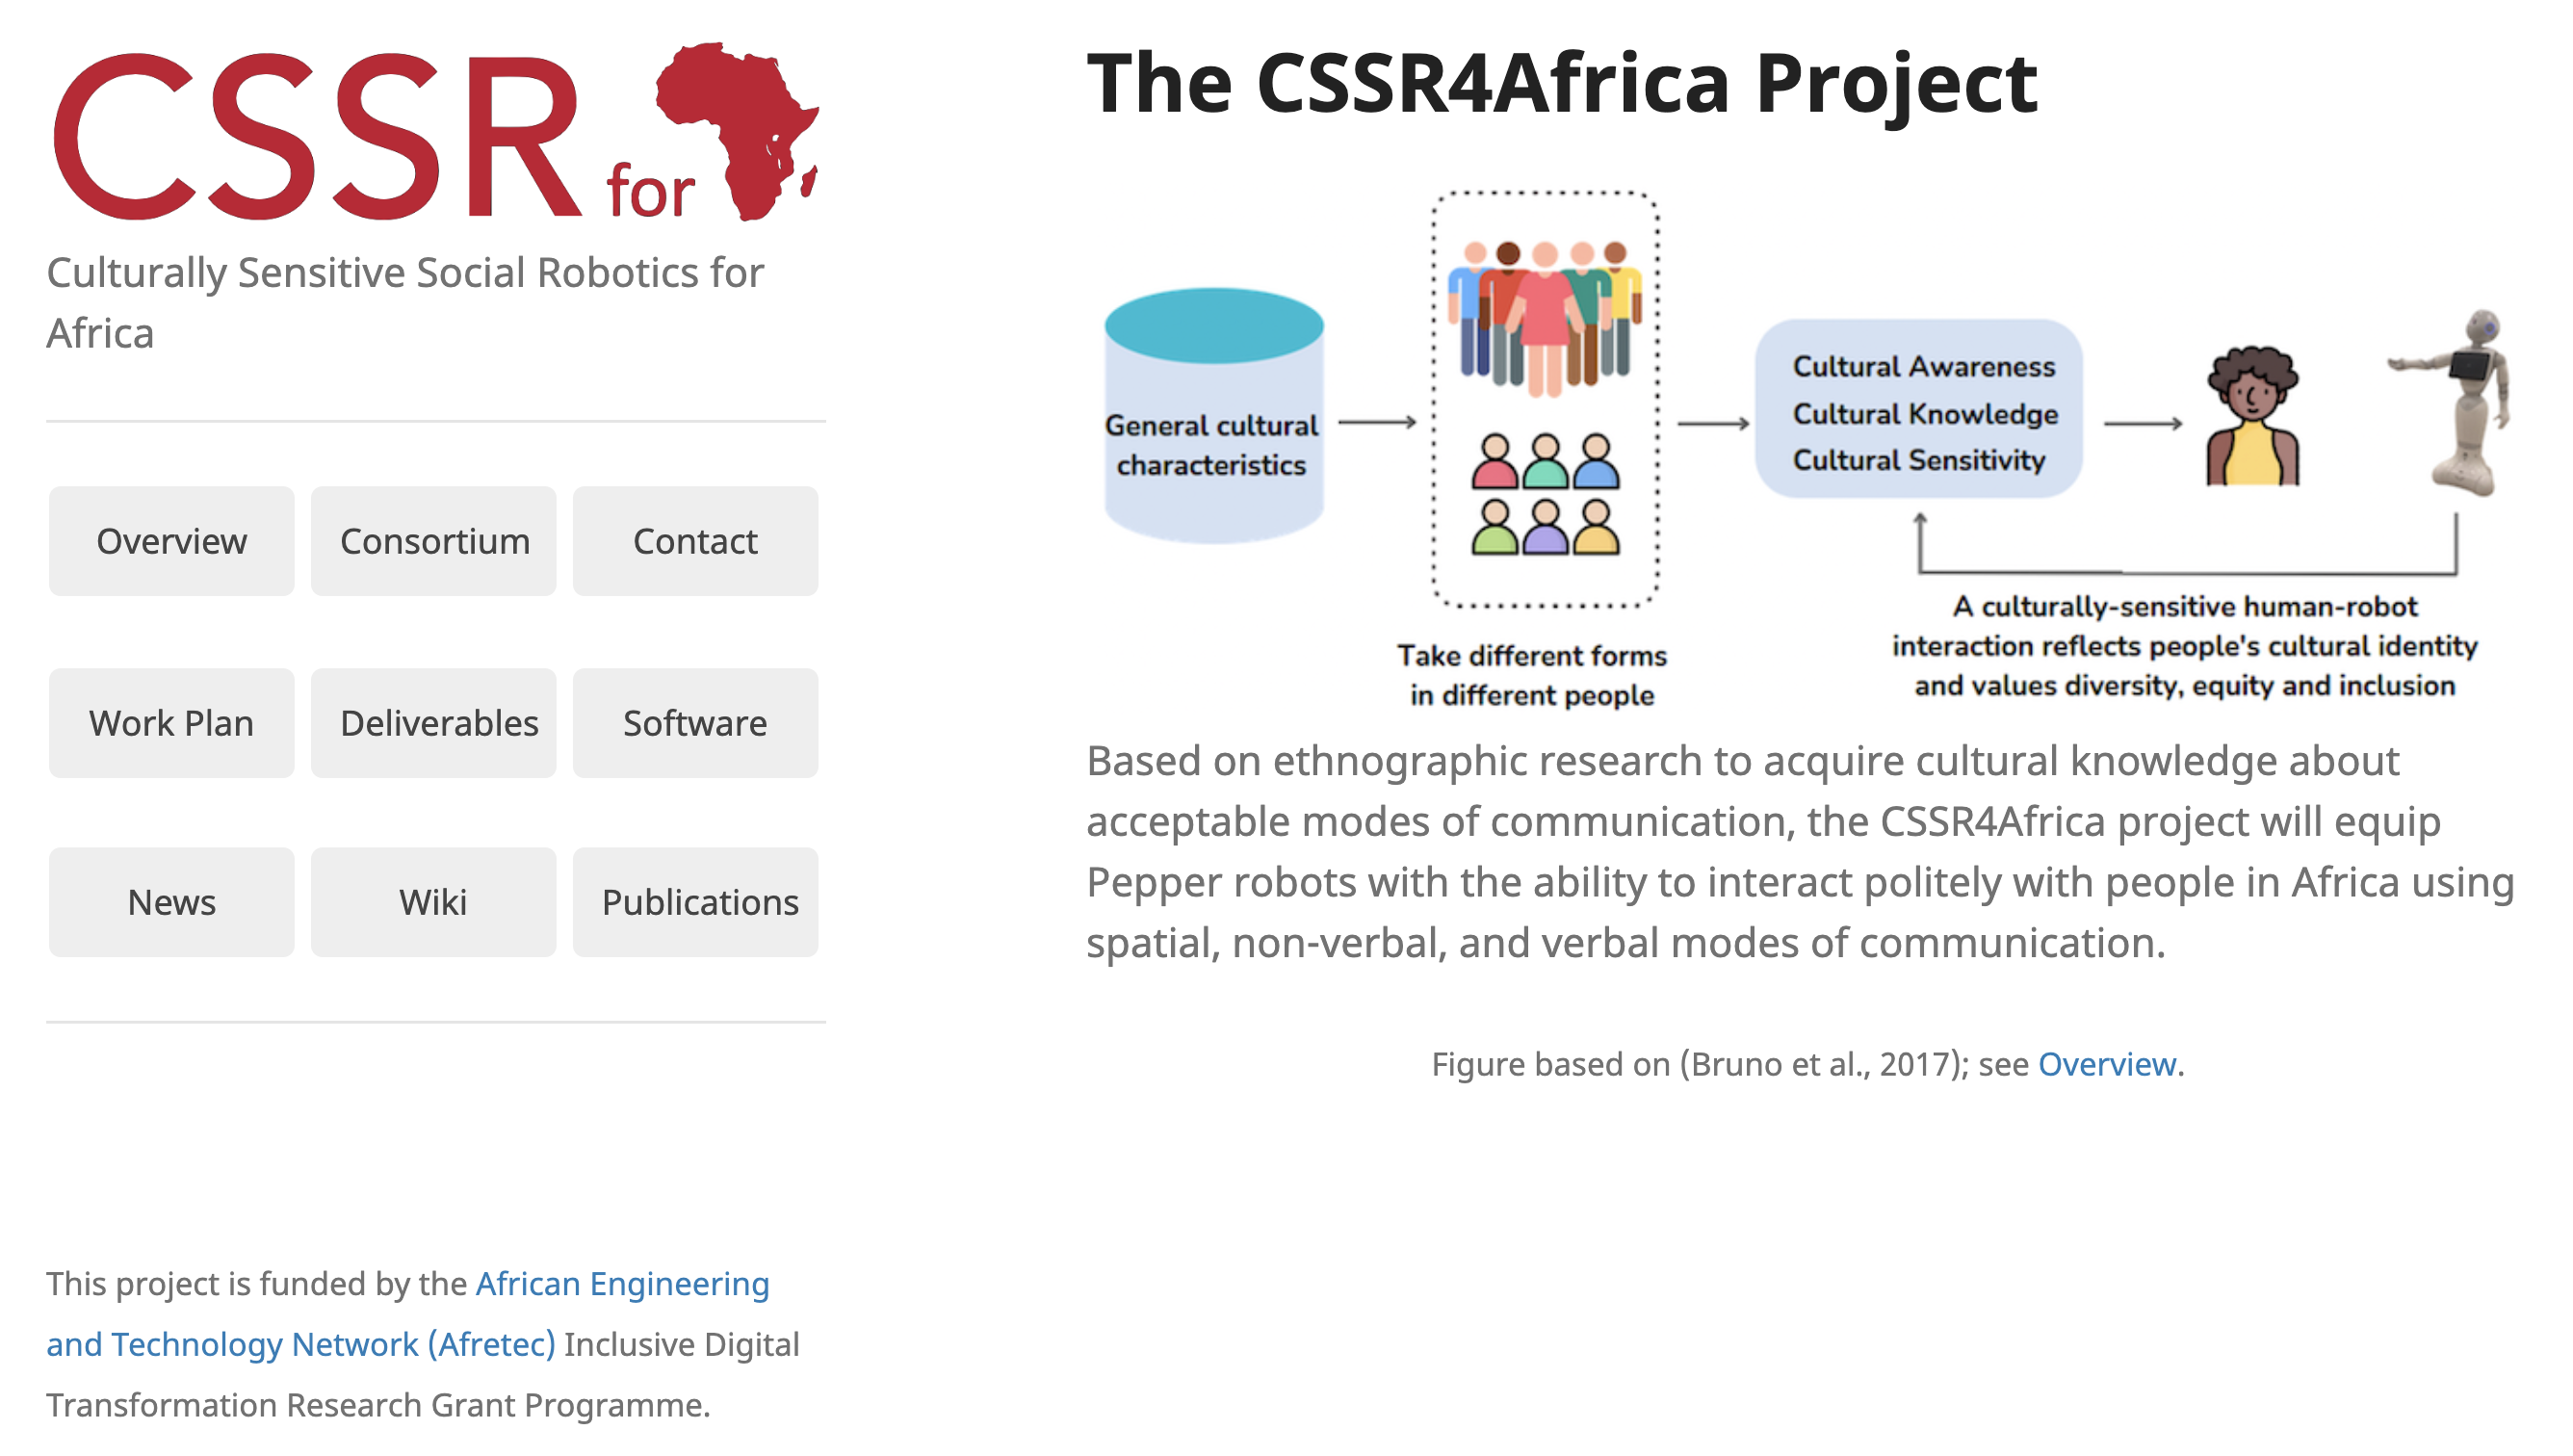
\includegraphics[width=140mm,angle=0]{./images/CSSR4Africa_website.png} 
\end{center}
\caption{Screenshot of the CSSR4Africa website.}          
\label{fig:website}                                                                
\end{figure}


The website is built using  Jekyll, a static site generator, on GitHub.   The layout is based on the Jekyll Minimal theme. This theme divides the page into two sections, one on the left and one on the right. The contents on the left appear on every page whereas the content on the right depends on the page that is being displayed; see Fig. \ref{fig:website}.

The left side comprises the CSSR4Africa logo and project title, nine clickable buttons which link to one external site and to eight pages that are displayed on the right side, and an acknowledgement line identifying the source of funding for the project.  The eight pages and one external site to which the buttons link are as follows. 

\begin{description}

\item[Overview] This page provides an overview of the CSSR4Africa project, including the motivation for cultural sensitivity in social robotics and an explanation of the difference between cultural sensitivity and cultural competence.

\item[Consortium]  This page identifies the two partners in the CSSR4Africa consortium: Carnegie Mellon University Africa and  University of the Witwatersrand, as well as links to the websites of the three principal investigators.

\item[Contact]  This page provides  the email addresses of the three principal investigators. The addresses are rendered in a manner that defeats web crawlers by rendering the ``@'' character as a png image.

\item[Work Plan]  This page provides a link to the CSSR4Africa work plan, comprising eight work packages, thirty-two tasks, and fourteen subtasks.

\item[Deliverables] This page provides links to the forty-two deliverables identified in the CSSR4Africa work plan.  A link to each deliverable is added to the page when the deliverables become available.

\item[Software] This page provides a link to the CSSR4Africa software repository on GitHub and a link to Deliverable D3.3 which describes the software installation process.
%% at \\{\small \url {https://github.com/cssr4africa/cssr4africa}}. 
This respository itself is described in Deliverable D7.3

\item[News] This page lists  notable events, reports, and deliverables.

\item[Wiki] This button takes you directly to the CSSR4Africa wiki, which is described in Section \ref{section:wiki}.

\item[Publications] This page lists all the papers that have been published in connection with the CSSR4Africa project, including those that were published prior to the official start date, and it provides links to PDF copies of each paper.

\end{description}


\subsection{Website Implementation}
%---------------------------------

\begin{figure}[thb]
\vspace{-1mm}
\centering
{\footnotesize
\begin{minipage}{5cm}
\dirtree{%
.1 docs.
.2 \_layouts.
.3 default.html.
.2 assets/css.
.3 style.scss.
.2 deliverables.
.2 images.
.2 meetings.
.2 publications.
.2 references.
.2 reports.
.2 resources.
.2 workplan.
.2 README.md.
.2 \_config.yml.
.2 consortium.md.
.2 contact.md.
.2 deliverables.md.
.2 favicon.ico.
.2 news.md.
.2 overview.md.
.2 publications.md.
.2 software.md.
.2 workplan.md.
}
\end{minipage}
}
\caption{The CSSR4Africa website directory structure and key files.}          
\label{fig:docs}                                                                
\end{figure}
 
\subsubsection{Directory Structure and Files}
%-------------------------------------
The website content is defined by a set of files in the {\small \texttt{docs}} directory of the CSSR4Africa GitHub Pages repository {\small \url {https://github.com/cssr4africa/cssr4africa.github.io}}.\footnote{GitHub Pages can be published from two directories, the root directory ({\small \texttt {/}}) and {\footnotesize\texttt{docs}}.}  The contents of the {\small \texttt{docs}} directory is shown in  Fig. \ref{fig:docs}.

The  {\small \texttt{default.html}} file in the {\small \texttt{\_layouts}} directory defines the appearance of the left side of the website, i.e., the header with the logo and project title, the array of menu buttons, and the acknowledgement of project funding.

The  {\small \texttt{style.scss}} file in the {\small \texttt{assets/css}} directory imports the Jekyll minimal theme and defines a new custom button style.

The   {\small \texttt{deliverables}} directory contains PDF copies of any deliverables published to date.

The   {\small \texttt{images}} directory contains any images used on the website, e.g., the organization logos, the CSSR4Africa logo, and diagrams.

The   {\small \texttt{meetings}} directory contains PDF copies of any material relating to project meetings and Afretec meetings.  This material is linked from the CSSR4Africa wiki, not the CSSR4Africa website.

The   {\small \texttt{publications}} directory contains PDF copies of any papers published by the CSSR4Africa partners.

The   {\small \texttt{references}} directory contains copies of key papers in the area of culturally sensitive robotics  that are not publicly available. This material is linked from the CSSR4Africa wiki, not the CSSR4Africa website.

The   {\small \texttt{reports}} directory contains the project's six-monthly periodic reports. This material is linked from the CSSR4Africa wiki, not the CSSR4Africa website.

The   {\small \texttt{resources}} directory contains any general resources that may be needed by the partners in the consortium, e.g., templates for deliverables and periodic reports. This material is linked from the CSSR4Africa wiki, not the CSSR4Africa website.

The   {\small \texttt{workplan}} directory contains a PDF copy of the latest version of the CSSR4Africa work plan.  

The   {\small \texttt{\_config.yml}} file defines theme to be used by Jekyll when building the website, i.e., the Jekyll minimal theme. It also defines a website title and description (in this case, the title of the project). This title appears alongside the page name in the browser's address bar and in a list of bookmarks.

The   {\small \texttt{favicon.ico}} file is a GIF image depicting the African continent in dark red. It appears in the browser's address bar and next to the page name in a list of bookmarks.

The   {\small \texttt{README.md}} file defines the content that appears on the right of the home page of the website. It is written using the Markdown markup language.

The {\small \texttt{consortium.md}}, {\small \texttt{contact.md}},  {\small \texttt{deliverables.md}},  {\small \texttt{news.md}},  {\small \texttt{overview.md}}, \\ {\small \texttt{publications.md}},  {\small \texttt{software.md}}, and {\small \texttt{workplan.md}}  files defines the contents of the consortium, contact, deliverables, news, overview, publications, software, and workplan pages. The content appears on the right side of the website when the respective button is clicked. They are written using the Markdown markup language.

\subsubsection{Publishing Content on the Website}
%-------------------------------------
All website content is developed locally and pushed to the GitHub website, as follows.

\begin{lstlisting}[style=Numbering, language=bash]
# Identify the files to be committed and put them in the staging area
# To select all new, deleted, or modified files, use git add . 
# To select a specific file, use git add ./<filename>
# Do this in the parent directory of the docs directory, 
# i.e., where the .git directory resides
git add .   

# Make these changes in the local repository
git commit -m "some message to identify the changes"

# Transfer the changed files to the remote repository on GitHub
git push origin main
\end{lstlisting}

Normally, the GitHub moderator publishes content provided by members of the consortium. If members of the consortium wish to publish content, they must first install git and clone the repository.  They will need the CSSR4Africa personal access token when logging in using the cssr4africa username. This can be provided by the  GitHub moderator. 

\newpage

\section{CSSR4Africa Wiki}
%----------------------
\label{section:wiki}


As noted above, the CSSR4Africa wiki is the forum used by the partners in the CSSR4Africa consortium to share information, documents, and data. Both wiki and website are public.  

\subsection{Wiki Address}
%----------------------

The wiki can be accessed from the CSSR4Africa website or directly at {\small \url{https://github.com/cssr4africa/cssr4africa.github.io/wiki/CSSR4Africa-Wiki}}.


\begin{figure}[tb]
\begin{center}
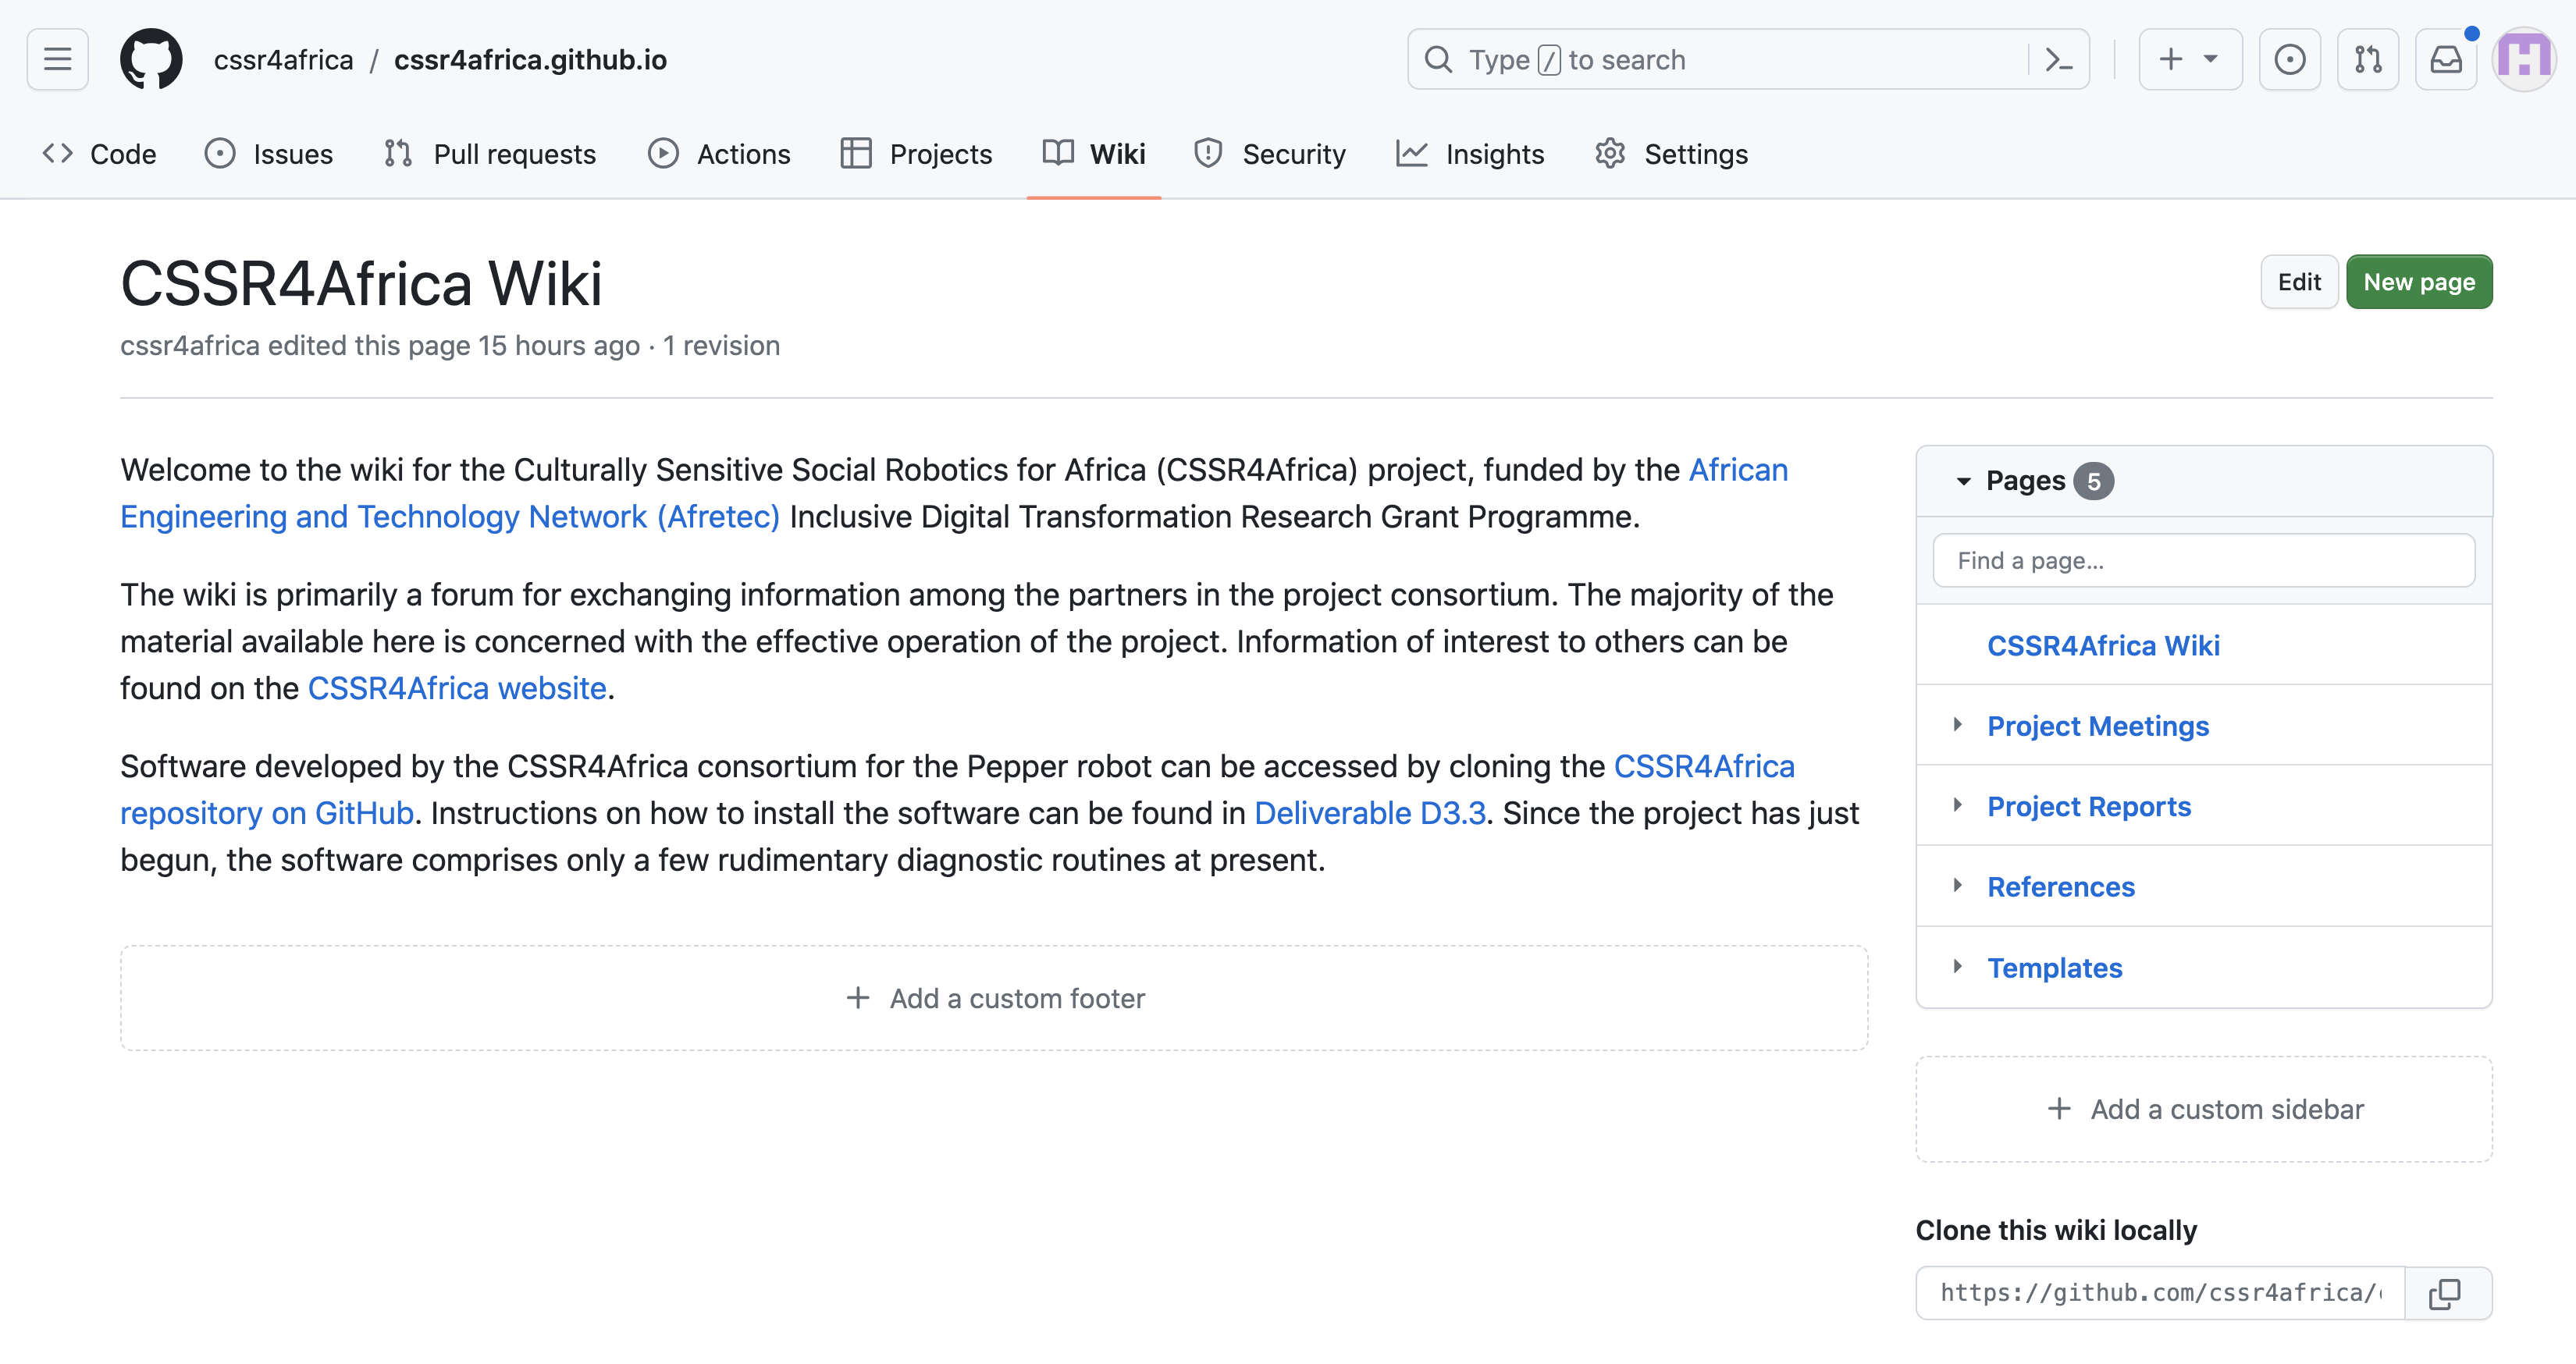
\includegraphics[width=160mm,angle=0]{./images/CSSR4Africa_wiki.png} 
\end{center}
\vspace{-5mm}
\caption{Screenshot of the CSSR4Africa wiki.}          
\label{fig:wiki}                                                                
\end{figure}

\subsubsection{Wiki Structure}
%------------------------

The structure of the wiki is dynamic by nature and it will grow and develop as the project progresses.  
At time of writing, it has five pages, as follows.
\begin{description}

\item[CSSR4Africa Wiki] This is the home page; see Fig. \ref{fig:wiki}.

\item[Project Meetings] This page lists the project meetings and  Afretec meetings, providing links to related material which is stored in the {\small \texttt{meetings}} directory.

\item[Project Reports] This page provides links to the six-monthly project periodic reports.  These  are stored in the {\small \texttt{reports}} directory.

\item[References] This page provides a list of  references to key publications in the area of culturally sensitive robotics, along with a  link to each paper.  Paper that are not publicly available are stored in the {\small \texttt{references}} directory.

\item[Templates] This page provides links to templates for periodic reports and deliverables.  These  are stored in the {\small \texttt{resources}} directory.

\end{description}


\subsubsection{Wiki Implementation}
%---------------------------------
GitHub repository wikis can use a variety of markup languages. The CSSR4Africa project has adopted the Markdown markup language for all its wiki pages.


\subsubsection{Publishing Content on the Wiki}
%---------------------------------------
Editing rights are restricted to collaborators who must be first be invited. Before being invited, they must sign up for a GitHub account,\footnote{For information on how to sign up for a GitHub account, see {\scriptsize \url {https://docs.github.com/en/get-started/signing-up-for-github/signing-up-for-a-new-github-account}}.} if they do not already have one, and send their username to the GitHub moderator. 



\newpage
\bibliographystyle{unsrt}
%================================================================
\bibliography{cognitive_systems.bib}                                     % REPLACE with correct filename
\addcontentsline{toc}{section}{References}



\pagebreak
\section*{Principal Contributors}
%===============================================================
\label{contributors}
\addcontentsline{toc}{section}{Principal Contributors}
The main authors of this deliverable are as follows (in alphabetical order).
\blank
~
\blank
Mihiretab Taye Hordofa, Carnegie Mellon University Africa.\\ 
David Vernon, Carnegie Mellon University Africa.\\   

  

\newpage
\section*{Document History}
%================================================================
\addcontentsline{toc}{section}{Document History}
\label{document_history}

\begin{description}

\item [Version 1.0]~\\
First draft. \\
David Vernon. \\                          
3 August 2023.                                    

\item [Version 1.0]~\\
Fixed several minor errors. \\
David Vernon. \\                          
7 August 2023.    

\end{description}

\end{document}

